\setlength{\intextsep}{3pt}
\renewcommand{\scalefigure}{0.4}
\begin{figure}[htbp]
	\centering
	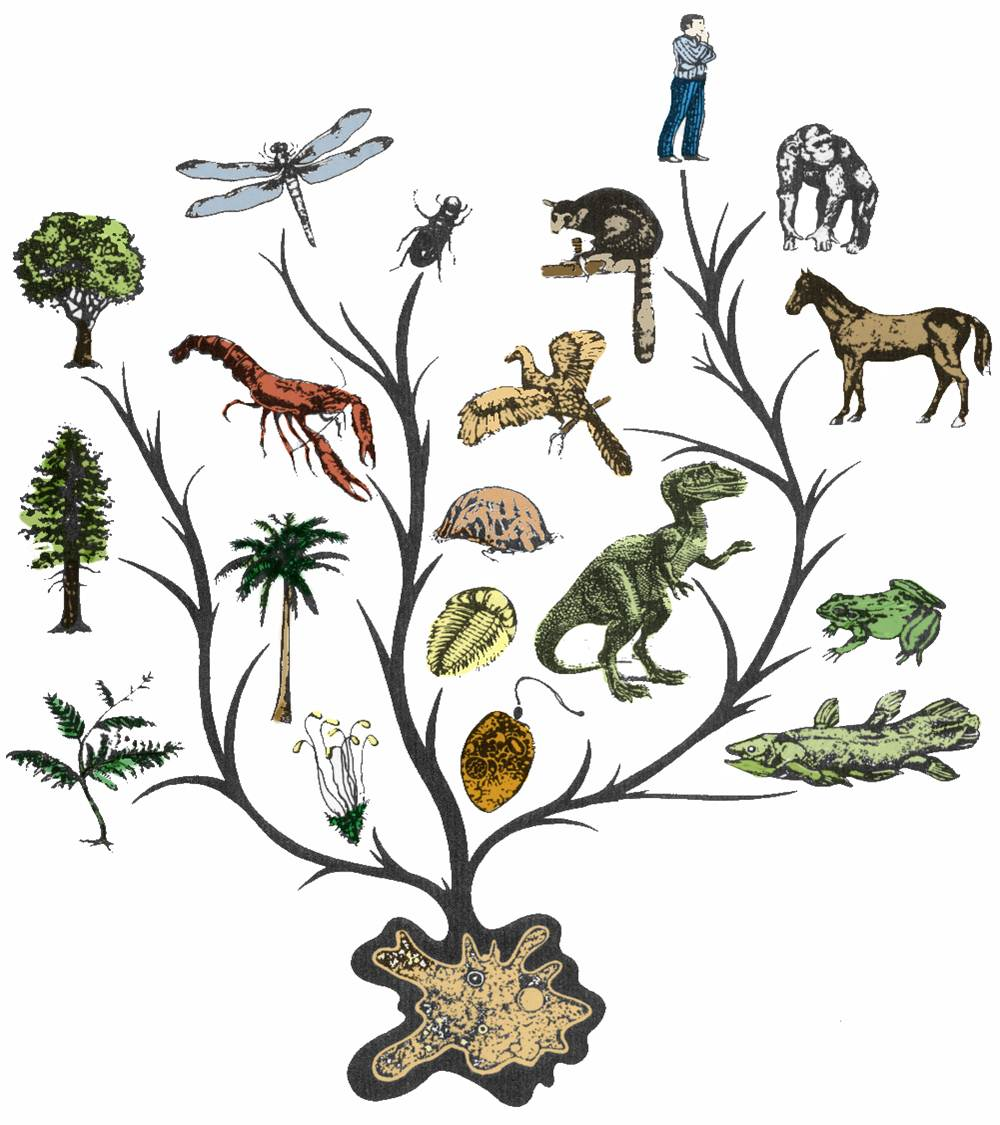
\includegraphics[scale=\scalefigure]{Figures/chap 1/evolution-tree.jpg}
	\label{fig:evolution_tree}
\end{figure}
\bigskip
\acrfull{ga} is one of the most popular representations of \gls{ea}. First proposed by John Holland in 1992~\cite{holland1992genetic}, \gls{ga} has been widely applied to solve a host of complex real-world problems as well as computationally theoretical ones. Inspired by Darwin's Theory of Evolution, the algorithm commences with a population of individuals that undergo reproduction to produce offspring. The procedure iterates itself intending to preserve genetic material, making a population fitter concerning a given environment while eliminating weaker individuals. The optimization of evolution progress guarantees that the next generation is always better than the previous one. Algorithm~\ref{alg:ga} shows the \gls{ga} framework, while details of this algorithm are presented in Subsection~\ref{ga:encoding} to~\ref{ga:terminate} as below.

\begin{algorithm}
	\caption{The skeleton of \gls{ga}}
	\label{alg:ga}
	\KwIn{An optimization problem}
	\KwOut{The best solution found for this problem}
	\BlankLine
	\Begin
	{	
		$P(0) \leftarrow$ Generate an initial population with $N$ individuals; \Comment{Refer to Subsection~\ref{ga:init}}\;
		\ForEach{individual $p_i$ in $P(0)$}
		{
			Evaluate the fitness of $p_i$; \Comment{Refer to Subsection~\ref{ga:fitness}}\;
		} 
		
		$t \leftarrow 1$\;
		\While{terminate conditions are not satisfied \Comment{Refer to Subsection~\ref{ga:terminate}}\;} 
		{
			$P'(t) \leftarrow$ Select the set of individuals from $P(t)$ for reproduction \Comment{Refer to Subsection~\ref{ga:selection}}\;
			$O(t) \leftarrow$ Generate an offspring population with $N$ individuals by using \emph{reproduction operators} on $P'(t)$; \Comment{Refer to Subsection~\ref{ga:reproduction}}\;
			\ForEach{individual $o_i$ in $O(t)$}
			{
				Evaluate the fitness of $o_i$\;
			} 
			$P(t+1) \leftarrow$ Select $N$ fittest individuals from $(P(t) \cup O(t))$ for the next generation\;
			$t \leftarrow t + 1$\;
		}
	}
\end{algorithm}

\subsection {Encoding Solutions - Chromosome}
\label{ga:encoding}
\gls{ga} utilizes a population of individuals, where each individual represents a candidate solution to the problem. The characteristics of an individual are represented by a chromosome, which can be partitioned into two types of evolutionary information~\cite{engelbrecht2007computational}: 
\begin{itemize}
	\item \textbf{Genotype:} A genotype is a term that represents an individual's genetic makeup as inherited from its parents. In other words, genotypes furnish a mechanism to preserve experiential evidence of previous generations.
	\item \textbf{Phenotype:} A phenotype is defined as the expressed behavioral traits of an individual in a given environment.
\end{itemize}

Genotype and phenotype always have a relationship with each other. When unexpected changes in phenotypic traits resulted from random gene alteration, it is called pleiotropy. In contrast, if a certain phenotypic trait is produced by the interaction of multiple genes, it is called polygeny. Generally, a chromosome consists of several genes, each representing a characteristic of the individual.

Encoding a solution is considered the most difficult step in \gls{ga}. This step requires an appropriate encoding such that each chromosome represents the corresponding solution to the real-world problem. There are several ways to represent a chromosome, for instance, a bit string.

\subsection {Fitness Function}
\label{ga:fitness}
The fitness function, which aims to map a chromosome into a scalar value, is pondered as the most crucial component of \gls{ga}. Because each chromosome represents a potential solution, the evaluation of the fitness function measures the quality of that chromosome. Furthermore, all evolutionary operators also make use of the fitness evaluation of chromosomes. For example, selection operators use the fitness value of each individual to select parents for reproduction. When determining a fitness function, we need to consider its practicability and implementation cost.

\subsection {Initial Population}
\label{ga:init}
The initialization process is the process of selecting individuals for the first population. The conventional method of forming the initial population is to choose gene values randomly from the allowed set of values. In many cases, based on available information about the search space, heuristic approaches can be applied to the initialization to take only potentially good solutions. Due to the large dimension of the search space, however, rarely all elements have a chance to be selected, which may cause premature convergence of the population to a local optimum. Therefore, the initial population's size plays an important role in performance in terms of accuracy and the time to converge.

\subsection {Selection Operators}
\label{ga:selection}
The selection operator takes the lead contribution to guarantee that the next generation of evolutionary progress is always better than the previous one. The new generation is generated basically through three operators, namely crossover, mutation, and elitism. In the case of crossover, the selection operator aims to choose fitter individuals to become parents. Similarly, the selection operator only nominates individuals with the lowest fitness values to be mutated in the mutation. Finally, the elitism operator retains a set of the fittest individuals to the next generation through the selection operator. 

In general, some of the most commonly used selection operators are:
\begin{itemize}
	\item \textbf{Random Selection:} All individuals are selected randomly. Therefore, they have an identical probability of getting chosen, whether they are good or terrible.
	\item \textbf{Roulette Selection:} The $i^{th}$ individual in the population has a probability of of getting chosen $p_i$ based on their fitness value $f(i)$ (Equation~\ref{eq:roullete}). Randomize a number $r$ between $[0,1]$. The $i^{th}$ individual is selected if $r < \sum^i_{k=1} f(k)$.
	\begin{equation}
		\label{eq:roullete}
		p_i = \frac{f(i)}{\sum^n_{n=1} f(i)}
	\end{equation}
	\item \textbf{Tournament Selection:} A certain number of individuals $k~(k > 0)$ are randomly selected and compared in pairs. The best individual among those $k$ individuals is then selected. The benefit of tournament selection is that the worst individuals will not be chosen, while the best individual will not dominate the reproduction process. 
	\item \textbf{Rank-Based Selection:} The likelihood of selection in rank-based selection is determined by the rank ordering of the fitness values rather than the fitness values themselves. As a result, ranking offers the advantage of preventing a highly fit individual from dominating the selection process.
\end{itemize}


\subsection {Reproduction Operators}
\label{ga:reproduction}
Crossover and mutation are two operators in reproduction that help with producing new offspring from selected parents. In the crossover, new offspring are created generally through the combination of two parents' genetic material. Some commonly used crossover operators can be mentioned, such as Two-point crossover, Order crossover, and Partially-mapped crossover. Depending on the characteristics of the problem to be solved, the crossover operators will be designed separately or modified accordingly.

The mutation, in contrast, randomly changes  the values in the chromosome gene. The crossover wishes to maintain dominant materials of parents to offspring, whereas mutation introduces new genetic material into the population. Some commonly used mutation operators include Swap mutation, Inversion mutation, and BitFlip mutation.

\subsection {Terminate Condition}
\label{ga:terminate}
An ideal terminate condition for \gls{ga} is when the individuals' fitness value reaches a pre-known optimal value of the objective function. However, the randomness of this algorithm makes it extremely difficult to satisfy the above condition, and in many cases, it can be impossible due to convergence. Therefore, other more commonly used typical termination conditions include: CPU time limit exceeded; Total number of population fitness evaluations reached a specific limit; Population diversity, or in other words, the convergence of the algorithm falls below a certain threshold.